\subsection{Real-Time Subsystem (RT subsystem)}

Contains modules responsible for the timekeeping. The components are internally connected
through WB crossbar (fig. \ref{fig:rts:hdl}) and controlled from Lattice Mico 32
and main CPU (through primary WB crossbar in the top design). Table
\ref{tab:rts:wb_base} contains Wishbone base address of each module inside the
Real-Time Subsystem.

\begin{figure}[ht]
  \begin{center}
    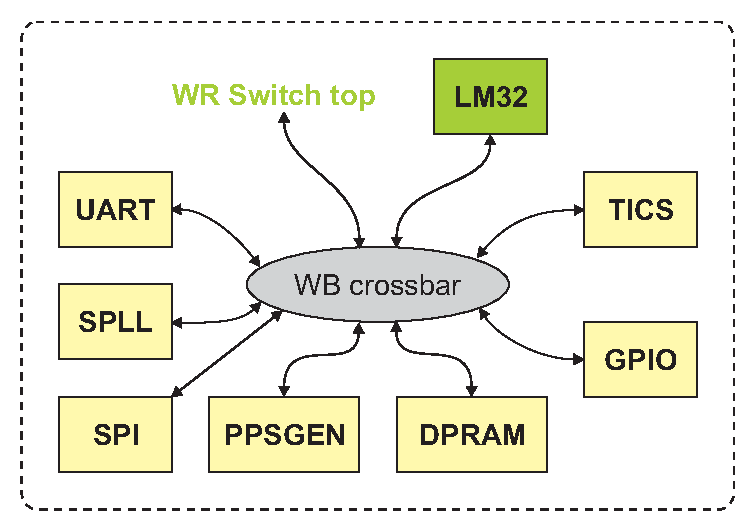
\includegraphics[width=.8\textwidth]{switch/rt_sub.pdf}
    \caption{Internal layout of Real-Time Subsystem block}
    \label{fig:rts:hdl}
  \end{center}
\end{figure}

\begin{table}[ht]
  \begin{center}
  \begin{tabular}{|l|l|}
    \hline
    module name & base address\\
    \hline \hline
    Dual-port RAM & 0x00000\\
    debug UART & 0x10000\\
    Soft-PLL & 0x10100\\
    SPI & 0x10200\\
    GPIO & 0x10300\\
    Timer block (TICS) & 0x10400\\
    1-PPS generator (PPSGEN) & 0x10500\\
    \hline
  \end{tabular}
  \caption{Wishbone base addresses of modules inside the Real-Time Subsystem}
  \label{tab:rts:wb_base}
  \end{center}
\end{table}

\subsubsection{LatticeMico32 (LM32)}
\noindent {\bf Description:}

Soft-core processor executing software implementation of PLLs (with
\emph{Soft-PLL} module).\\

\noindent{\bf Wishbone interface:}

\emph{LM32} is a Wishbone Master, does not have any WB configuration registers.

\subsubsection{Dual-port RAM (DPRAM)}
\noindent {\bf Description:}

Instruction and data memory for \emph{LM32} soft-core processor
controlling \emph{Soft-PLL}. It has to be programmed with \emph{LM32} binary
from the main CPU when the WR Switch boots.

\subsubsection{Debug UART}
\noindent {\bf Description:}

UART driven by \emph{LM32}, outputs debug information from Software PLLs.\\

\noindent{\bf Wishbone interface:}

Only \emph{LM32} talks to this interface, WR Switch software does not access it.

\subsubsection{Soft-PLL (SPLL)}
\noindent {\bf Description:}

HDL part of Soft-PLL implementation. Controlled over Wishbone from \emph{LM32}
software.\\

\noindent{\bf Wishbone interface:}

Only \emph{LM32} talks to this interface, WR Switch software does not access it.

\subsubsection{SPI}
\noindent {\bf Description:}

Used by software running on \emph{LM32} to adjust the tunable oscillators (part
of SoftPLL implementation).\\

\noindent{\bf Wishbone interface:}

Only \emph{LM32} talks to this interface, WR Switch software does not access it.

\subsubsection{GPIO}
\noindent {\bf Description:}

Controls GPIO lines through Wishbone interface. All of the signals currently
used are output-only. They are mostly (besides GPIO2) driven from \emph{LM32}
software as part of SoftPLL algorithm implementation.

Signals controlled by the module:

\begin{center}
  \begin{tabular}{|l|l|l|p{8cm}|}
    \hline
    {\bf GPIO No.} & {\bf direction} & {\bf used by} & {\bf description}\\
    \hline
    \hline
    0 & output & \emph{LM32} & selects system clock for FPGA modules to be a startup clock (0) or the
    clock coming from from PLL (1) i.e. aligned to WR time\\
    1 & output & \emph{LM32} & resets AD9516 clock generator\\
    2 & output & \emph{WR Switch SW} & active high reset of \emph{LM32} softcore, used by
    the \emph{LM32} firmware loader while it is being stored to DPRAM\\
    3 & output & \emph{LM32} & active low reset of WR Switch peripherals (Endpoint,
    Switching Core, Topology Resolution Unit, GTX Ser/Des, Tx Timestamping Unit,
    GPIO port of top design, $I^2C$ master interfaces, Per-port Statistics)\\
    4 - 31 & && not used\\ %\multicolumn{3}{l|}{not used}\\
    \hline
  \end{tabular}
\end{center}

\noindent{\bf Wishbone interface:} section \ref{subsec:wbgen:gpio}.

\subsubsection{Timer block}
\noindent {\bf Description:}

Used by \emph{LM32} for counting time intervals independent from the local
timebase (being adjusted).\\

\noindent{\bf Wishbone interface:}

Only \emph{LM32} talks to this interface, WR Switch software does not access it.

\subsubsection{1-PPS generator}
\noindent {\bf Description:}

The module is responsible for generating and inputting 1-PPS signal. It
contains two timekeeping counters: \emph{cntr\_utc} and \emph{cntr\_nsec}. The
former keeps full seconds of the White Rabbit time, while the latter represents
fractional part of each second. \emph{cntr\_nsec} is clocked with 62.5 MHz
reference clock which means that its granularity is 16 ns. The 1-PPS pulse is
generated at the beginning of each second i.e. \emph{cntr\_nsec} equals to 0.

Wishbone registers of 1-PPS generator allow modifications of \emph{cntr\_utc}
and \emph{cntr\_nsec} counters. It can be performed in two ways: setting or
adjusting the time. The former simply stores new values to the counters when
requested. The adjustment is done by adding new values to the current state of
the counters (\emph{cntr\_utc}, \emph{cntr\_nsec}) at the beginning of a new second (when \emph{cntr\_nsec} is 0).\\

\noindent{\bf Wishbone interface:} section \ref{subsec:wbgen:ppsg}.
